\begin{singlespacing}
\chapter{The \atlas\ Experiment}
\label{chapter:experiment}
%
\begin{epigraphs}
\qitem{%
if observing outer space gives us a view of the past, observing inner space
would surely give us a glimpse into the future - would be interesting if NASA
made a telescope for that%
}%
{Ken~M,
\textit{Comment: Yahoo! News},
2012~\cite{kenm2012inner}}
\end{epigraphs}
\end{singlespacing}
\noindent
Towards explaining the main result of this thesis,
a search for effects from supersymmetric models
in data from the \atlas\ detector
on the Large Hadron Collider (LHC)~\cite{
atlas2022searches,
atlas2008experiment,
lhc2008machine
},
we first cover some relevant facts about the design and motivations
behind \atlas.

The \atlas\ detector was not delivered in a preordained form.
It was designed with intent to provide maximally useful and novel data within
real-world budgets.
Alongside ambitions for general-purpose utility, \atlas's designs aimed to
construct a detector that could
\begin{itemize}
\item find the Higgs boson (which was predicted but yet unseen),
\item precisely measure known massive objects ($W$, $Z$, and $t$), and possibly
\item discover new (supersymmetric) particles~\cite{atlas1999design1}.
\end{itemize}
We review these three goals with news \atlas's subsequent operations.

\paragraph{Find the Higgs boson.}
Before \atlas's construction, the Higgs boson mass (and existence) was
uncertain, but loosely constrained by results like
$m(h) \gtrsim 90\,\eV[G]$ from searches at the
Large Electron–Positron Collider (LEP),
$m(h) = 76^{+85}_{-47}\,\eV[G]$ from other data on the electroweak sector,
and $m(h) \lesssim 1\,\eV[T]$ from unitarity arguments~\cite{
atlas1999design2,
ghinculov1998perturb,
lep1999ewk
}.

The Higgs boson couples to an extraordinary variety of fundamental particles.
For its discovery alone, \atlas's designers achieved sensitivity across the
entire $100\,\eV[G]$ to $\,\eV[T]$ window by targetting decays including
$h \to b\bar b$,
$h \to \gamma\gamma$,
$h \to ZZ^* \to 4\ell$, and
$h \to ZZ \to \ell\ell\nu\nu$.
These channels demand precise measurements of leptons, photons, and
$b$-jets (jets seeded by $b$ quarks), as well as sensitivity to the missing
transverse momentum of invisible neutrinos.

\atlas\ and \cms\ have now found a Higgs boson candidate with
$m(h) = 125\,\eV[G]$~\cite{
atlas2012higgs,
atlas2012combined,
cms2012higgs
}
and confirmed all of its tested Standard Model properties~\cite{
combined2016higgs,
atlas2022ten,
cms2022ten
}
such as its production mechanisms, decay rates,
spin, and parity~\cite{
HIGG-2013-01,
HIGG-2013-17,
HIGG-2014-06
}.

\paragraph{Precisely measure known massive objects.}
Other than the Higgs boson, the heavy Standard Model resonances are the
$W$ and $Z$ bosons and the top quark.
All of these are produced at high rates in LHC proton-proton collisions,
and present opportunities for \atlas\ to measure their properties
(such as masses and production cross-sections) with unprecedented precision.

Sensitivity to hadronic momenta is crucial,
both directly to measure heavy hadronic decays
(like $t \to bq\bar{q}$),
and indirectly for the missing transverse momenta from semi-invisible
leptonic decays (like $W \to \ell\nu$).
Since individual hadron identities are less relevant to these measurements,%
\footnote{%
Rare decays like
$W^\pm \to \pi^\pm \gamma$ or $W^\pm \to \pi^\pm \pi^+ \pi^-$
could give clean signals, but are not competitive due to their
tiny cross-sections~\cite{
cdf1996search,
mangano2014wpiy,
cms2021wpiy
}.
Leptonic $B$ hadron decays are useful for $m(t)$ measurements, but do not
require hadron identification~\cite{
CDF:2009mbf,
CMS:2016ixg,
ATLAS:2022jbw
}.%
}
it makes sense for \atlas's design to forfeit hadron identification systems
in favour of precise calorimetry with total angular coverage.

\atlas\ has now produced a plethora of competitively precise measurements
of the heaviest particles in the Standard Model~\cite{atlas2021summarysm},
including $m(W)$~\cite{atlas2018wmass} and
$m(t)$~\cite{atlas2022symmarytop, atlas2019topmass, TOPQ-2015-03},
but also details of differential cross-sections~\cite{
STDM-2016-11,
STDM-2016-14,
TOPQ-2018-15,
TOPQ-2016-10
}.
Rare processes have also been studied in new levels of detail,
including
electroweak diboson ($WW/WZ/ZZ$ etc.)~\cite{
STDM-2015-21,
STDM-2015-23,
STDM-2017-09
}
and triboson~\cite{
STDM-2016-06,
STDM-2017-22,
STDM-2019-09
},
and rare top processes
($\ttbar Z$, $\ttbar W$ etc.)~\cite{
TOPQ-2013-05,
TOPQ-2018-01,
TOPQ-2020-03
}.
These measurements continue to refine the Standard Model, and their precision
is aided by no new phenomena getting in the way.

\paragraph{Discover new (supersymmetric) particles.}
High-energy proton-proton collisions at the LHC offer sensitivity
to new particles up to multi-$\eV[T]$ mass scales.
Heavy new particles are anticipated to either decay to known Standard Model
objects, or to be invisible in \atlas.
Designs that can discover such new particles are therefore neatly aligned with
our other goals of refining the current Standard Model
and to discovering the Higgs boson.
Visible decay products should already be caught by \atlas's abilities
to measure the Higgs boson and other Standard Model particles,
and the prospect of new invisible particles reinforces the need for precise
measurements of the missing transverse momentum.

Indeed, the main search of this thesis~\cite{atlas2022searches}
meets nicely with the pre-existing need for sensitivity to signatures
including
$h \to b\bar b$
and
$ZZ \to \ell\ell\nu\nu$.
Dozens of searches for new phenomena have now been conducted in \atlas\ data,
with and without supersymmetry~\cite{
ATL-PHYS-PUB-2022-013,
ATL-PHYS-PUB-2022-007,
ATL-PHYS-PUB-2022-012,
ATL-PHYS-PUB-2022-036,
ATL-PHYS-PUB-2022-034
},
and show no convincing sign of effects beyond the Standard Model.
This is not a failure. It is a success.
Our scientific goal is not to discover something that is not there,
but to learn more about nature.
Discovering no tangible new particles in LHC conditions is itself a discovery.

Without high-energy hadron collisions in its centre, \atlas\ would be neutered.
We are therefore indebted to the LHC for so reliably providing the exciting
hadron collisions that are necessary for all of our proton collision data.
We therefore begin this chapter with a description of the LHC itself in
Section~\ref{sec:atlas_lhc}, before detailing the design of \atlas\ in
Section~\ref{sec:atlas_design}.

\section{The Large Hadron Collider}
\label{sec:atlas_lhc}

% the LHC
% where the protons come from
Figure~\ref{fig:experiment_cern_complex}

\begin{figure}[tp]
\centering
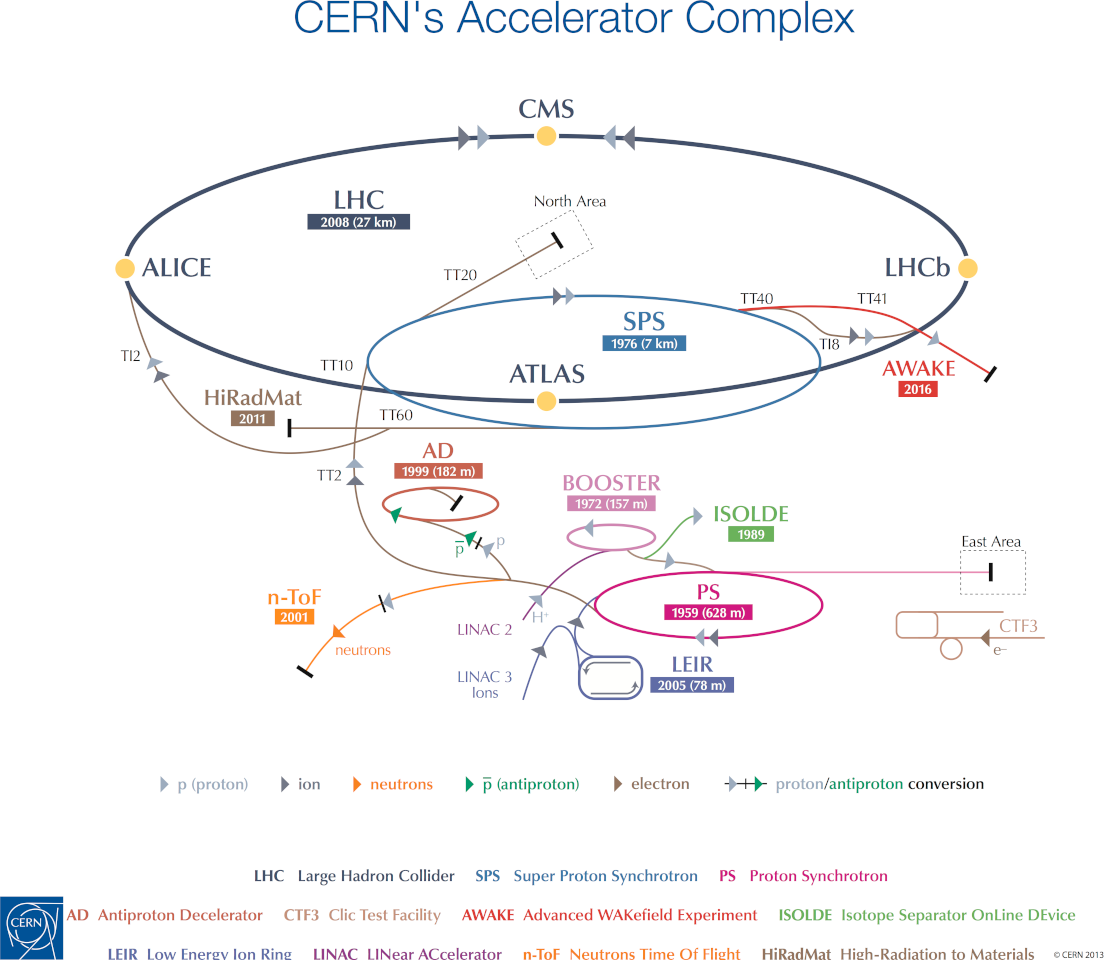
\includegraphics[width=0.99\textwidth]{figures/atlas_lhc_complex.png}
\caption[
The CERN accelerator and detector complex, with the LHC as its largest piece
]{%
The CERN accelerator and detector complex, with the LHC as its largest piece
shown in dark blue-grey.
The complex uses a sequence of increasingly large and powerful accelerators to
boost ionised particles to their final collision energies in the LHC and to
yield beams for other CERN experiments.
This poster is adapted from~\cite{Haffner:1621894}.
}
\label{fig:experiment_cern_complex}
\end{figure}

% the accelerator complex
% - sequence of contributing accelerators and their beam energies
% beampipe restricted by size of lep tunnel
% - required particle count makes antiprotons hard
% - proton-proton same charge requires separate beampipes
% - size means most cost efficient to put both beams in one cryostat
% - beampipes therefore mechanically and magnetically coupled
% - superconducting magnets at around 2 to 4 Kelvin
% - cooled with superfluid helium
% - low heat capacity, danger of heating from beam radiation
% Radiofrequency cavities
% - radio waves at 400 MHz such that slow protons accelerated, fast decelerated
% - in LHC, accelerates from 450 GeV to 6.5 TeV (7 target)
% magnets
% - dipole for steering
% - quadrupole for focussing (pairs)
% - higher orders why? septupole at beam entry
% size of beam
% luminosity and its uncertainty
% pile-up
\TODO{Distribution in the mean number of primary vertices per crossing, where the
variability in that mean arises from differing beam conditions over run-time.}
Figure~\ref{fig:experiment_run_2_mu}

\begin{figure}[tp]
\centering
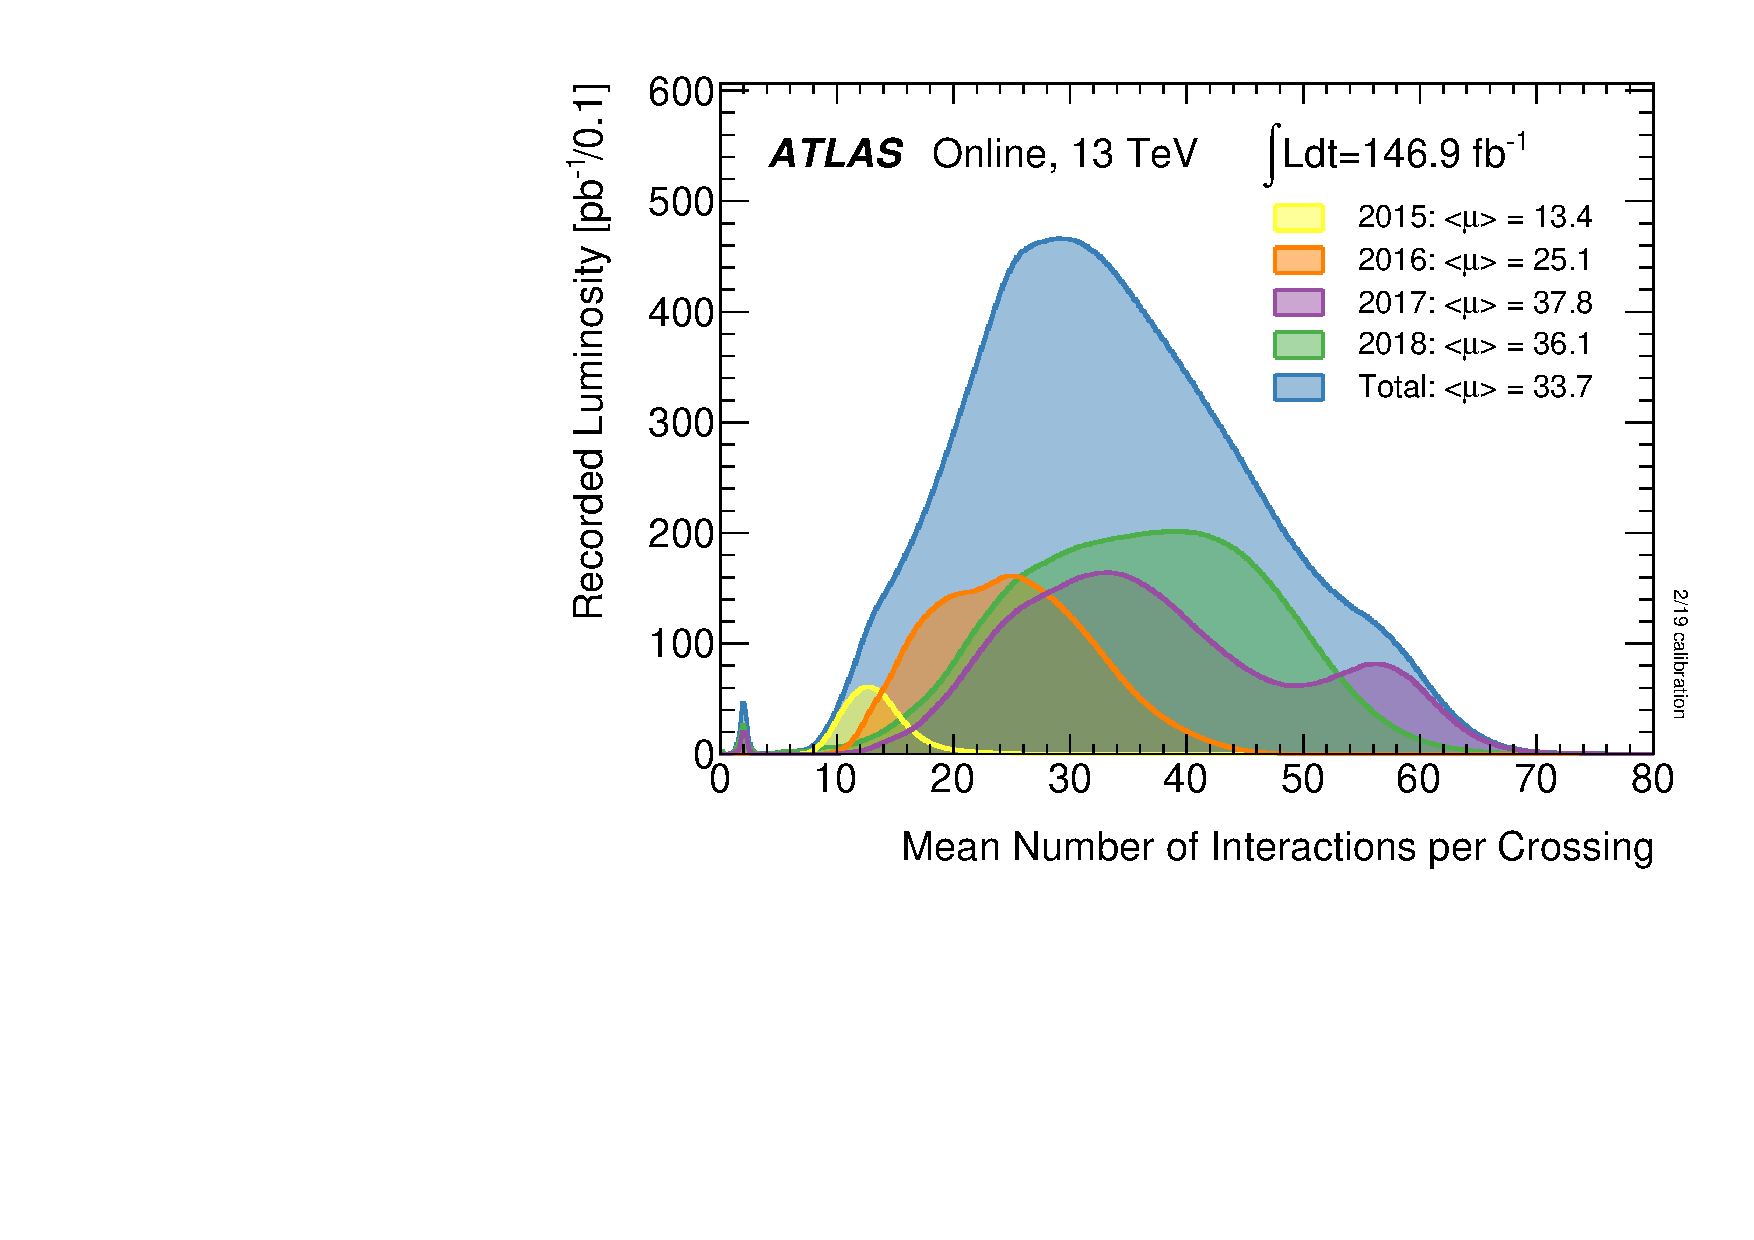
\includegraphics[width=0.62\textwidth]{figures/atlas_pileup_mu_2015_2018.pdf}
\caption[
Mean number interactions per bunch crossing in Run~2 of the LHC
]{%
Mean number interactions per bunch crossing in Run~2 of the LHC;
rates presented are weighted by luminosity and sub-divided by year of
operation.
This figure includes all data that \atlas\ recorded with stable LHC proton
beams.
The reported integrated luminosities therefore exceed those we present later
in Table~\ref{tab:experiment_run2_state}, which are further filtered to require
other data-goodness criteria.
This figure is reproduced from~\cite{atlas_public_luminosity}.
}
\label{fig:experiment_run_2_mu}
\end{figure}


\section{Design}
\label{sec:atlas_design}
Atlas is a Titan.
\atlas\ is the largest detector experiment at the LHC,
and alongside its biggest neighbours
\cms~\cite{cms2008experiment},
\lhcb~\cite{lhcb2008experiment},
and ALICE~\cite{alice2008experiment}
it is a multi-kilotonne beast,
and a wonder of scientific engineering~\cite{
atlas1994proposal,
atlas2008experiment,
atlas1999design1,
atlas1999design2
}.

\begin{figure}[tp]
\centering
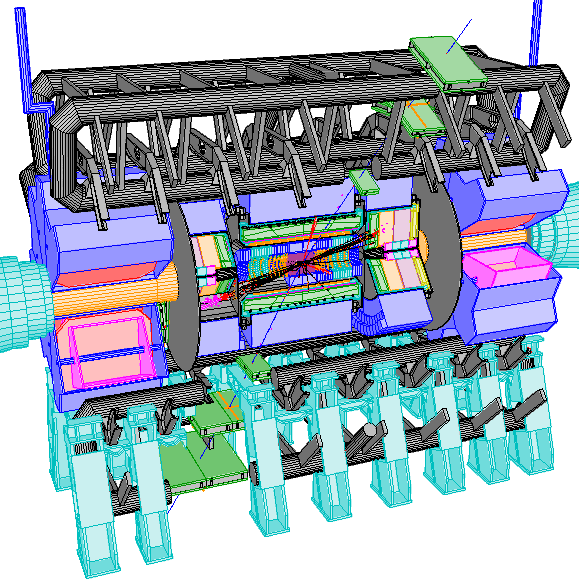
\includegraphics[width=0.62\textwidth]{figures/atlas_cutaway_volume_1.pdf}
\caption[
A central slice of \atlas's design
]{%
A central slice of \atlas's design, reproduced from~\cite{atlas1999design1,
persint2014manual},
including a simulated event that interacts with several sensitive subsystems.
}
\label{fig:atlas_cutaway}
\end{figure}

Our search paper~\cite{atlas2022searches} contains concise and standard
descriptions of the \atlas\ detector and its relevant components.
Through its evolution in many past \atlas\ publications, these descriptions
have become so highly refined that attempts to improve them myself would
probably be in vain.
Instead, this section quotes our published text with explanatory commentary.
\begin{quote}
``%
The ATLAS detector~\cite{atlas2008experiment} is a multipurpose particle
detector with a forward--backward symmetric cylindrical geometry and a near
$4\pi$ coverage in solid angle.%
\footnote{%
``ATLAS uses a right-handed coordinate system with its origin at the nominal
interaction point (IP) in the centre of the detector and the $z$-axis along the
beam pipe.
The $x$-axis points from the IP to the centre of the LHC ring, and the $y$-axis
points upwards.
Cylindrical coordinates $(r,\phi)$ are used in the transverse plane, $\phi$
being the azimuthal angle around the $z$-axis.
The pseudorapidity is defined in terms of the polar angle $\theta$ as
$\eta = -\ln \tan(\theta/2)$.
Angular distance is measured in units of
$\Delta R \equiv \sqrt{(\Delta\eta)^{2} + (\Delta\phi)^{2}}$.%
''\footnotemark~\cite{atlas2022searches}%
}
It consists of an inner tracking detector surrounded by a thin superconducting
solenoid providing a $2\,\mathrm{T}$ axial magnetic field, electromagnetic and
hadronic calorimeters, and a muon spectrometer.%
''~\cite{atlas2022searches}
\end{quote}
To illustrate this summary, Figure~\ref{fig:atlas_cutaway} shows a vertical slice
of \atlas.
Each subsystem is described in more detail in a subsection below:
the inner tracking detector in Section~\ref{sec:atlas_inner},
the electromagnetic and hadronic calorimeters in
Section~\ref{sec:atlas_calo},
and
the muon spectrometer in Section~\ref{sec:atlas_muon}.
These detectors' resolutions to relevant physical objects is described in
Section~\label{sec:atlas_object_resolutions}.
The final connection to data analysed in this thesis is made through the
trigger system, which is described in Section~\ref{sec:atlas_trigger},
and details of the data themselves are given in
Section~\ref{sec:atlas_data}.

\footnotetext{%
This footnote appears in every \atlas\ publication, but was perfected
in~\cite{lester2013heffalon}.
True to form, internal \atlas\ guidelines request that
``If you think you can improve on it, please consult with the
Publications Committee''~\cite{atlas_coordinate, atlas_footnote}.
}


\section{Inner detector}
\label{sec:atlas_inner}
The inner tracking detectors begin \atlas's measurements of new collisions
by precisely tracing the paths taken by energetic charged particles
as they curve through the solenoidal magnetic field.
Track curvature provides momentum information,
tracks' associations into collision vertices helps to separate the multiple
scatterings per crossing (pile-up),
and their associations into displaced vertices help to identify
decays.
\begin{quote}
``%
The inner tracking detector covers the pseudorapidity range $|\eta| < 2.5$.
It consists of silicon pixel, silicon microstrip, and transition radiation
tracking detectors.
An additional layer of silicon pixels, the insertable
B-layer~\cite{ATLAS-TDR-19, PIX-2018-001}, was installed before Run~2.%
''~\cite{atlas2022searches}
\end{quote}
This insertable B-layer is a silicon pixel detector that begins just
$3\,\textrm{cm}$ from the beam-pipe, and provides robust tracking for the
high luminosity of the current LHC,%
\footnote{%
Instantaneous luminosity in the Run~2 LHC peaked at
$19\times10^{33}\,\mathrm{cm}^{-2}\mathrm{s}^{-1}$ in 2018~\cite{ATLAS:2022hro},
which is much higher than previous conditions such as the Run~1 peak
instantaneous luminosity of
$3.6\times10^{33}\,\mathrm{cm}^{-2}\mathrm{s}^{-1}$ in 2012~\cite{ATLAS:2013tpw}.
The future High-Luminosity LHC (HL-LHC), however, might achieve
$75\times10^{33}\,\mathrm{cm}^{-2}\mathrm{s}^{-1}$.
For the HL-LHC, the current inner tracking and insertable B-layer will
be replaced by a new Inner Trac\emph{k}er (ITk) which is designed to handle such
extreme luminosity conditions~\cite{CERN-LHCC-2017-021}.
}
particularly for sensitivity to particles whose lifetimes are just right to
decay inside the tracking system;
these `Goldilocks Zone' particles include B-hadrons, some tau leptons, and
maybe new species.

Following radially outwards are the silicon pixel and silicon microstrip%
\footnote{%
Formerly known as the SemiConductor Tracker~\cite{atlas1999design1},
the silicon microstrip system retains the acronym
SCT~\cite{atlas2008experiment}.%
}
detectors (which use silicon technology)
and the transition radiation tracking detector
(which uses `straw' gas tubes).

As for the whole \atlas\ detector, complete $\phi$ coverage and a large $\eta$
range minimizes leakage from the inner detector.
Towards design goals, this tracking detector provides crucial
measurements of electrons and B-hadrons,
and contributes to the reconstruction of missing transverse momentum.


\section{Calorimeters}
\label{sec:atlas_calo}
Inelastic collisions cause energetic particles to scatter, distributing their
energy into macroscopic particle showers.
Calorimetry uses this principle to measure energies
by interleaving dense absorbing materials (which initiate showers)
with sensitive materials that convert showers into electrical signals.
In \atlas,
\begin{quote}
``%
Lead/liquid-argon (LAr) sampling calorimeters provide electromagnetic (EM)
energy measurements with high granularity.
A steel/scintillator-tile hadron calorimeter covers the central pseudorapidity
range ($|\eta| < 1.7$).
The end-cap and forward regions are instrumented with LAr calorimeters for both
the EM and hadronic energy measurements up to $|\eta| = 4.9$.%
''~\cite{atlas2022searches}
\end{quote}
The electromagnetic calorimeters provide located electron/photon energy
measurements,
and the hadronic calorimeters subsequently aim to stop and measure hadronic
activity for later analysis in jet clustering.
Maximal angular coverage by the calorimeters further facilitates missing
transverse momentum measurements.

Neither `A' in \atlas\ stands for Argon, but perhaps one could.
Liquid-argon is the chosen active material in the electromagnetic and forward
calorimeters for its robust, linear response in converting showers to
electrical signals for readout by electrodes.
Liquid argon is poured as a liquid to fill the gaps between the various
metallic absorbers, which are folded into zigzag ``accordion'' shapes that
optimize uniformity around the detector.
The steel/scintillator hadronic tile calorimeter is a
``simple and cost effective''~\cite{atlas1996tile} design, which uses
photomultiplier tubes to convert light from its polystyrene scintillators into
electrical signals.
Particles lose some energy before reaching the calorimeters; a thin
liquid-argon pre-sampler is installed before the central EM calorimeter
to regain these losses.

The calorimeter systems achieve attenuations of at least ten interaction
lengths throughout their $|\eta| < 4.9$ range;
by maximizing this attenuation, the design minimizes noise from hadronic
`punch-through' of non-muons into the muon system.


\section{Muon system}
\label{sec:atlas_muon}
Muons penetrate matter well because of their large mass and non-interaction
with the strong nuclear force.
\atlas\ doesn't try to stop energetic muons;
above around $3\,\eV[G]$, they pass right through the calorimeters, and are
instead measured by their curved tracks in a toroidal magnetic field that
permeates dedicated muon detectors on \atlas's periphery.
\begin{quote}
``%
The muon spectrometer surrounds the calorimeters and is based on three large
superconducting air-core toroidal magnets with eight coils each.
The field integral of the toroids ranges between $2.0$ and
$6.0\,\mathrm{T\kern-0.15ex m}$ across most of the detector.
The muon spectrometer includes a system of precision chambers for tracking and
fast detectors for triggering.%
''~\cite{atlas2022searches}
\end{quote}
Muon subsystems come in four varieties, all of which operate by detecting
charges scattered by the muons as they fly through gaseous media.
Together, these systems track the muons' paths as the magnets bend them in the
longitudinal plane; these toroidal magnets generate fields outside the tile
calorimeter around the central barrel and in the end-caps as illustrated in
Figure~\ref{fig:atlas_magnets}.

\begin{figure}[tp]
\centering
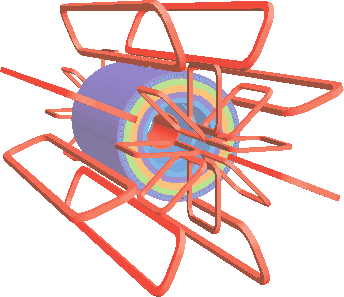
\includegraphics[width=0.62\textwidth]{figures/atlas_magnets.pdf}
\caption[
Layout of \atlas's toroidal magnets around the tile calorimeter and inner
solenoid
]{%
Layout of \atlas's toroidal magnets around the tile calorimeter and inner
solenoid, including the eight barrel and end-cap coils,
reproduced from~\cite{atlas2008experiment}.
The \atlas\ muon spectrometer measures muons' tracks as they bend through
this peripheral magnetic field.
}
\label{fig:atlas_magnets}
\end{figure}

Measurements of the tracks' curvature yield estimates of the muons' momenta;
although extremely energetic muons will have straight tracks,
\atlas's construction and calibration achieves a high precision which
loosens to only $10\%$ relative error on tracks with $1\,\eV[T]$ transverse
momenta~\cite{
atlas1994proposal,
atlas2008experiment,
ATL-PHYS-PUB-2015-037
}.


\section{Object resolutions}
\label{sec:atlas_object_resolutions}
Ultimately, the majority usage of most of \atlas's data happens through their
reconstructions into interpretable objects, such as muons, electrons, jets,
photons, or taus.
From one perspective, these reconstructions are themselves exact data, as they
are nothing less than functions of observed data.
However, reconstructed objects do not exactly coincide with some proposed
underlying truth --- reconstructions more closely resemble that truth perturbed
by some noise.
\atlas's experimental resolution determines the scale of that noise.

Since the $\twoljets$ analysis is most concerned with muons, electrons and
jets and missing transverse momentum,
this section reviews \atlas's experimental resolutions for these objects.

\paragraph{Muons.}
Since hard muons are not stopped inside \atlas, their reconstruction derives
from the curved tracks they leave in the inner detector and muon system as they
traverse \atlas's strong magnetic fields.
High tracking fidelity allows us to reliably reconstruct muons across most of
their expected momentum spectrum, with $\sigma(\pt) / \pt \lesssim 10\%$ up to
$\pt \approx 1\,\eV[T]$.
But resolution must degrade as these tracks' curvatures reduce at very high
energies, and Figure~\ref{fig:atlas_cutaway} illustrates this degradation.
The relative momentum resolution is approximately Gaussian in
$1 / \pt$ for muons across this momentum range
(and therefore non-Gaussian in $\pt$ itself)~\cite{atlas1999design1}.

\begin{figure}[tp]
\centering
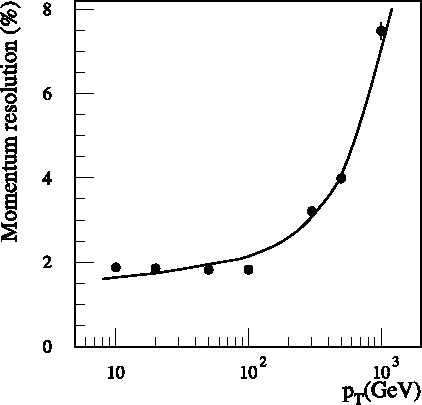
\includegraphics[width=0.8\textwidth]{figures/atlas_muon_resolution.pdf}
\caption[
Relative muon momentum resolution in \atlas\ as a function of $\pt$
]{%
Relative muon momentum resolution in \atlas\ as a function of $\pt$, for
muons selected within a pseudorapidity window of $|\eta| < 1.5$ and averaged
over that window.
The dots mark resolution values extracted from simulations, and the line
represents a semi-empirical description of the relative
resolution~\cite{CERN-LHCC-97-022}.
This figure is reproduced from~\cite{atlas1999design1}.
}
\label{fig:atlas_cutaway}
\end{figure}

At a reference transverse momentum of $\pt = 100\,\eV[G]$, \atlas's typical
relative muon momentum resolution is at the $\sigma(\pt) / \pt \approx 2\%$
level.
However, non-uniformities in the detector geometry cause this to spike up to
$\approx 10\%$ in local areas of the $\eta\textrm{--}\phi$ angular space;
these degraded local areas include regions containing cryostat hardware or
the detector's supporting feet~\cite{atlas1999design1, CERN-LHCC-97-022}.


\paragraph{Electrons.}
Electrons are measured by both tracking in the inner detector and calorimetry
in the electromagnetic calorimeter.
These two measurements give two complementary inputs that aid in electron
reconstruction.
As for muons, the resolution from tracking scales with $1/\pt$, but the
calorimetry error is dominated by Poisson statistics with a number of charged
particles that scales in proportion to the electron's energy.
Combining these two factors with a constant baseline noise, one can therefore
model the relative electron resolution as
\begin{equation}
\label{eqn:experiment_electron_resolution}
\frac{\sigma(\pt)}{\pt}
\approx
\frac{a_1}{\sqrt{\pt}}
\oplus
\frac{a_2}{\pt}
\oplus
a_3
,
\end{equation}
in which $\oplus$ indicates a sum in quadrature.
To describe \atlas, these $a_i$ parameters are roughly
$a_1 \approx 0.1\,\sqrt{\eV[G]}$,
$a_2 \approx 0.25\,\eV[G]$, and
$a_3 \approx 0.007$~\cite{nackenhorst2010top, Lester:705139, ERDMANN201418}.
Although resolutions vary across the solid angle, this formula roughly
reproduces the reported electron resolutions of
$\frac{\sigma(\pt)}{\pt} \approx 4\%$ at $\pt = 10\,\eV[G]$,
$\frac{\sigma(\pt)}{\pt} \approx 1\%$ at $\pt = 100\,\eV[G]$, and
$\frac{\sigma(\pt)}{\pt} \approx 0.1\%$ at
$\pt = 1\,\eV[T]$~\cite{atlas2019electron}.

Energy losses from high-energy electrons are dominated by Bremsstrahlung
radiations, in which the electron radiates a photon and recoils from its
momentum.
Electron reconstruction algorithms efficiently recover this lost Bremsstrahlung
momentum by associating nearby photon calorimeter clusters back to their source
electron many cases~\cite{atlas1994proposal, atlas1999design1}.

\paragraph{Jets.}
Although charged hadrons are tracked in the inner detector, the total energy of
jets also depends vitally on neutral hadrons, which are only observed through
their hadronic interactions in the calorimeter system.
With less influence from tracking, calorimetry noise is the dominant
contribution to the experimental resolution on hadronic jets.
However, other noise contributions arising from electrical signals and pile-up
scale in proportion in $1/\pt$.
one can therefore again approximate \atlas's relative jet energy resolution as
\begin{equation}
\label{eqn:experiment_jet_resolution}
\frac{\sigma(\pt)}{\pt}
\approx
\frac{b_1}{\sqrt{\pt}}
\oplus
\frac{b_2}{\pt}
\oplus
b_3
,
\end{equation}
the same functional form as for electrons in
Equation~\ref{eqn:experiment_electron_resolution},
with
$b_1 \approx 1.0\,\sqrt{\eV[G]}$
$b_2 \approx 0.5\,\eV[G]$, and
$b_3 \approx 0.03$.
With these parameters, formula approximately describes the measured relative
jet resolutions of
$\frac{\sigma(\pt)}{\pt} \approx 20\%$ at $\pt = 30\,\eV[G]$,
$\frac{\sigma(\pt)}{\pt} \approx 8\%$ at $\pt = 200\,\eV[G]$, and
$\frac{\sigma(\pt)}{\pt} \approx 4\%$ at
$\pt = 2\,\eV[T]$~\cite{atlas2021jetresolution}.

Note that hadronic weak decays can produce real, not-prompt missing momentum
in jets.
This effect can skew jet reconstruction distributions towards low energies,
and is particularly prominent for heavy-flavour jets~\cite{nackenhorst2010top}.

\paragraph{Missing transverse momentum.}
Measurement resolutions of all other objects propagate into the missing
transverse momentum; this is necessary as it is not directly observed itself,
but derived from other objects' transverse momenta.
But collisions also emit significant amounts of momentum in softer particles,
which can leave tracks and calorimeter hits without being clustered into hard
physical objects such as jets or electrons.
The $\met$ resolution therefore depends not only on the resolutions of hard
objects, but also on the measurement of this soft contribution.
Various different $\met$ definitions, known as `working points', use different
quality criteria to define the $\met$ composition, and each working point
balances resolution against accuracy for different context-specific
objectives~\cite{ATLAS-CONF-2018-023, Pacey:2747774}.

Pile-up is a major contributor to the $\met$ resolution, because secondary
interactions produce both tracks and calorimeter clusters that might can be
indistinguishable from products of the hard-scatter primary vertex
(the main interaction of interest in a bunch crossing).
All misattributed momentum from these additional vertices causes $\met$ noise.
The \atlas\ $\met$ resolution is reported in two orthogonal transverse
components: $\sigma(\metx)$ and $\sigma(\mety)$.%
\footnote{%
The directional decomposition of $\ptmiss$ uncertainty is important for the
$\met$ significance variable $\metsig$, which we shall discuss in
Section~\ref{sec:2ljets_metsig}.
}%
\footnote{%
Despite their $E$ symbols, these variables $\metx$ and $\mety$ are momenta
because they have spatial directions.%
}
In reference samples of simulated $Z \to \mu\mu$ events, both transverse
$\met$ resolution components increase with the number of primary vertices in a
bunch crossing ($n_{PV}$), from
$\sigma(\metx) = \sigma(\mety) \approx 10\,\eV[G]$ at $n_{PV} = 1$, to
$\sigma(\metx) = \sigma(\mety) \approx 20\,\eV[G]$ at $n_{PV} = 30$.
Note that these resolutions vary by around $\pm 20\%$ with the $\met$
working point choice~\cite{ATLAS-CONF-2018-023}.


\section{Trigger}
\label{sec:atlas_trigger}
The LHC's $25\,\mathrm{ns}$ time difference between proton bunches
(bunch spacing) is so fast that light-speed particles ejected from one crossing
are still zipping through \atlas's $12.5\,\textrm{m}$ radius when the next
collision arrives.
This extreme engineering is necessary to achieve the integrated luminosities we
need to see rare effects, but to avoid becoming overwhelmed
by data it also demands a strict data reduction mechanism.
This mechanism is the trigger:
\begin{quote}
``%
A two-level trigger system is used to select events.
The first-level trigger is implemented in hardware and uses a subset of the
detector information to accept events at a rate below $100\,\mathrm{kHz}$.
This is followed by a software-based trigger that reduces the accepted event
rate to $1\,\mathrm{kHz}$ on average depending on the data-taking conditions.%
''~\cite{atlas2022searches}
\end{quote}
The first-level (L1) trigger uses its fast preliminary information to accept
interesting events, and mark regions of interest.
A Region-of-Interest (RoI) is an angular region of a detector subsystem.
Each RoI is assigned in $\eta\textrm{--}\phi$ coordinates to contain detector materials
that should contain more data on the effects seen in L1.
RoI sizes vary from
$\Delta\eta \times \Delta\phi \approx 0.1 \times 0.1$ for electron/photon
reconstruction, up to
$\Delta\eta \times \Delta\phi = 0.8 \times 0.8$ for
hadronic jets~\cite{atlas2016trigger}.
Complete data in the regions of interest are passed to the second-level
(high-level trigger, HLT) to inform its decision of whether to accept each
event.
To reduce processing time, HLT algorithms can choose to inspect data only in,
or near to, each regions of interest.
Events accepted by the HLT are recorded for future analysis~\cite{
atlas2016trigger,
atlas2008experiment
}.

\atlas\ implements a menu of many different triggers for specific categories of
interesting events in a representative time period.
This trigger menu includes triggers for combinations of up to three charged
leptons, one or two photons, up to six jets, up to two $b$-tagged jets, missing
transverse momentum, or hadronic states for $B$ physics.
Of these, Table~\ref{tab:experiment_trigger_breakdown} summarises the most
important trigger categories and their trigger rates under peak Run~2
operations.
In total, the peak HLT trigger rate was $1750\,\mathrm{Hz}$ for the main
physics categories, and $200\,\mathrm{Hz}$ for the $B$-physics trigger category
(which also triggers on other, non-$B$, light
states)~\cite{ATL-DAQ-PUB-2019-001}.
The $\twoljets$ search presented in this thesis uses only dilepton triggers
for electrons and muons.
As shown in Table~\ref{tab:experiment_trigger_breakdown}, these have a total
HLT trigger rate less than $105\,\mathrm{Hz}$%
\footnote{%
The listed rates overlap, so the sum of their peak rates is only an upper
bound on their union.
},
meaning that our chosen triggers cover only a few percent of \atlas's data.

\begin{table}[tp]
\centering
\footnotesize
\begin{adjustbox}{width=\textwidth}
\begin{tabular}{llcc}
Trigger                        & Summary                                                          & L1 Peak Rate ($\mathrm{kHz}$) & HLT Peak Rate ($\mathrm{Hz}$) \\
\hline
\multirow{5}{*}{Single lepton} & Isolated $\mu$, $\pt > 27\,\eV[G]$                               & $16$                          & $218$                         \\
                               & Isolated tight $e$, $\pt > 27\,\eV[G]$                           & $31$                          & $195$                         \\
                               & $\mu$, $\pt > 52\,\eV[G]$                                        & $16$                          & $70$                          \\
                               & $e$, $\pt > 61\,\eV[G]$                                          & $28$                          & $20$                          \\
                               & $\tau$, $\pt > 170\,\eV[G]$                                      & $1.4$                         & $42$                          \\
\hline
\multirow{9}{*}{Dilepton}      & \textbf{$\mu\mu$, both $\pt > 15\,\eV[G]$}                       & \textbf{$2.2$}                & \textbf{$30$}                 \\
                               & \textbf{$\mu\mu$, $\pt > 23, 9\,\eV[G]$}                         & \textbf{$16$}                 & \textbf{$47$}                 \\
                               & \textbf{loose $ee$, both $\pt > 18\,\eV[G]$}                     & \textbf{$2.0$}                & \textbf{$13$}                 \\
                               & \textbf{$e\mu$, $\pt > 18, 15\,\eV[G]$}                          & \textbf{$16$}                 & \textbf{$6$}                  \\
                               & \textbf{loose $e$, $\mu$, $\pt > 18, 15\,\eV[G]$}                & \textbf{$2.6$}                & \textbf{$5$}                  \\
                               & \textbf{$e\mu$, $\pt > 29, 9\,\eV[G]$}                           & \textbf{$21$}                 & \textbf{$4$}                  \\
                               & $\tau\tau$, $\pt > 40, 30\,\eV[G]$                               & $5.7$                         & $93$                          \\
                               & $\tau$, isolated $\mu$, $\pt > 30, 15\,\eV[G]$                   & $2.4$                         & $17$                          \\
                               & $\tau$, isolated $e$, $\pt > 30, 18\,\eV[G]$                     & $4.6$                         & $19$                          \\
\hline
\multirow{5}{*}{Trilepton}     & loose $eee$, $\pt > 25,13,13\,\eV[G]$                            & $1.6$                         & $0.1$                         \\
                               & $\mu\mu\mu$, $\pt > 7\,\eV[G]$                                   & $0.2$                         & $7$                           \\
                               & $\mu\mu\mu$, $\pt > 21,5,5\,\eV[G]$                              & $16$                          & $9$                           \\
                               & $\mu\mu$, loose $e$, $\pt > 11,11,13\,\eV[G]$                    & $2.2$                         & $0.5$                         \\
                               & loose $ee$, $\mu$, $\pt > 13,13,11\,\eV[G]$                      & $2.3$                         & $0.1$                         \\
\hline
Single photon                  & loose $\gamma$, $\pt > 145\,\eV[G]$                              & $24$                          & $47$                          \\
\hline
\multirow{3}{*}{Diphoton}      & loose $\gamma\gamma$, both $\pt > 55\,\eV[G]$                    & $3.0$                         & $7$                           \\
                               & $\gamma\gamma$, $\pt > 40,30\,\eV[G]$                            & $3.0$                         & $21$                          \\
                               & isolated tight $\gamma\gamma$, both $\pt > 25\,\eV[G]$           & $2.0$                         & $15$                          \\
\hline
\multirow{3}{*}{Single jet}    & jet ($R = 0.4$), $\pt > 435\,\eV[G]$                             & $3.7$                         & $35$                          \\
                               & jet ($R = 1.0$), $\pt > 480\,\eV[G]$                             & $2.6$                         & $42$                          \\
                               & jet ($R = 1.0$), $\pt > 450\,\eV[G]$, $m_j > 45\,\eV[G]$         & $2.6$                         & $36$                          \\
\hline
\multirow{5}{*}{$b$-jet}       & $b$-tag @ $60\%$, $\pt > 285\,\eV[G]$                            & $3.6$                         & $15$                          \\
                               & two $b$-tag @ $60\%$, $\pt > 185,70\,\eV[G]$                     & $3.6$                         & $11$                          \\
                               & $b$-tag @ $60\%$, three jets, all $\pt > 85\,\eV[G]$             & $1.5$                         & $14$                          \\
                               & two $b$-tag @ $60\%$, one jet, $\pt > 65, 65,160\,\eV[G]$        & $1.3$                         & $17$                          \\
                               & two $b$-tag @ $60\%$, two jets, all $\pt > 65\,\eV[G]$           & $3.2$                         & $15$                          \\
\hline
\multirow{4}{*}{Multi-jet}     & four jets, all $\pt > 125\,\eV[G]$                               & $0.5$                         & $16$                          \\
                               & five jets, all $\pt > 95\,\eV[G]$                                & $4.8$                         & $10$                          \\
                               & six jets, all $\pt > 80\,\eV[G]$                                 & $4.8$                         & $4$                           \\
                               & six jets, all $|\eta| < 2$, all $\pt > 60\,\eV[G]$               & $4.8$                         & $15$                          \\
\hline
$\met$                         & $\met > 200\,\eV[G]$                                             & $5.1$                         & $94$                          \\
\hline
\multirow{4}{*}{$B$-physics}   & $\mu\mu$, $\pt > 11, 6\,\eV[G]$, $0.1 < m_{\mu\mu} < 14\,\eV[G]$ & $2.9$                         & $55$                          \\
                               & $\mu\mu$, $\pt > 6, 6\,\eV[G]$, $2.5 < m_{\mu\mu} < 4.0\,\eV[G]$ & $1.4$                         & $55$                          \\
                               & $\mu\mu$, $\pt > 6, 6\,\eV[G]$, $4.7 < m_{\mu\mu} < 5.9\,\eV[G]$ & $1.4$                         & $6$                           \\
                               & $\mu\mu$, $\pt > 6, 6\,\eV[G]$, $7 < m_{\mu\mu} < 12\,\eV[G]$    & $1.2$                         & $12$
\end{tabular}
\end{adjustbox}
\caption[
Summary of \atlas\ trigger rates in 2018 data
]{%
Summary of \atlas\ trigger rates in 2018 data at the peak instantaneous
luminosity of $2\times10^{34}\,\mathrm{cm}^{-2}\mathrm{s}^{-1}$.
The search presented in this thesis uses only dilepton $e$ and $\mu$ triggers,
which are highlighted in bold.
Table adapted from~\cite{ATL-DAQ-PUB-2019-001}.
Rates overlap between triggers.
}
\label{tab:experiment_trigger_breakdown}
\end{table}

\section{Data}
\label{sec:atlas_data}
Raw binary data are hard for us humans to interpret.
Before use in publishable analysis projects, software systems first mutate
those data into a workable form, of clean events with calibrated and
interpretable event variables.
\begin{quote}
``%
An extensive software suite~\cite{ATL-SOFT-PUB-2021-001} is used in the
reconstruction and analysis of real and simulated data, in detector operations,
and in the trigger and data acquisition systems of the experiment.%
''~\cite{atlas2022searches}
\end{quote}
Prediction is important in data analysis.
This software suite helps to generate predictive simulations, and provides
realism by passing both the real and simulated data through the same processing
pipelines~\cite{SOFT-2010-01, geant2003}.
Software models of the \atlas\ detector itself are refined with the results from
many calibration studies and in-situ measurements~\cite{atlas2008experiment},

The search of this thesis uses data from proton-proton collisions at
$\sqrt{s} = 13\,\eV[T]$ centre-of-mass energies in Run~2 of the
LHC, in which \atlas\ collected data in the years
$2015\textrm{--}2018$~\cite{atlas2022searches}.
This second run has various refinements over the Run~1, including beam energies
increasing from $\sqrt{s} = 7\textrm{ or }8\,\eV[T]$, and bunch spacings
halving from $50$ to $25\,\textrm{ns}$~\cite{lhc2006run2}.
A breakdown of the LHC proton-proton data conditions and quantity is given
in Table~\ref{tab:experiment_run2_state}.
Broadly, instantaneous luminosity was increased over time, leading to increases
in both data quantity and pile-up interactions alongside those data.

\begin{sidewaystable}[tp]
\centering
\begin{tabular}{lcccc}
Observable                                                        & 2015         & 2016         & 2017                & 2018         \\
\hline
Maximum number of colliding bunch-pairs                           & $2232$       & $2208$       & $2544$ ($1909$)     & $2544$       \\
Bunch spacing ($\mathrm{ns}$)                                     & $25$         & $25$         & $25$ (variable)     & $25$         \\
Typical number of protons per bunch ($\times 10^{11}$)            & $1.1$        & $1.1$        & $1.1$ ($1.2$)       & $1.1$        \\
Peak luminosity ($\times 10^{33}\mathrm{cm}^{-2}\mathrm{s}^{-1}$) & $5$          & $13$         & $16$                & $19$         \\
Peak number of inelastic interactions per crossing                & $\approx 16$ & $\approx 41$ & $\approx 45$ ($60$) & $\approx 55$ \\
Luminosity-weighted average inelastic interactions per crossing   & $13$         & $25$         & $38$                & $36$         \\
Integrated luminosity delivered ($\mathrm{fb}^{-1}$)              & $4$          & $39$         & $50.6$              & $63.8$
\end{tabular}
\caption[
LHC data rates and conditions by year in Run~2
]{%
LHC data rates and conditions by year in Run~2.
This table is adapted from~\cite{ATLAS:2022hro}.
Bracketed numbers under 2017 refer to an alternative `8b4e' LHC operating
condition which alternated in a pattern of eight bunches with the usual
$25\,\mathrm{ns}$ separation followed by a gap of four empty bunch slots.
Alongside a primary interaction, the inelastic interactions in a crossing are
pile-up events and add noise to our measurements.
}
\label{tab:experiment_run2_state}
\end{sidewaystable}

Data collected under anomalous detector operations are hard to model.
Lists are maintained indicating which datasets arise from `good', normal
detector operations, and these lists are commonly employed to select only clean
subsets of good data for analysis projects.
Testament to the quality of \atlas's operations, this cleaning removes less
than $5\%$ of the Run~2 data~\cite{
DAPR-2018-01,
Golling:2011zy
}.
After selecting for data quality requirements, we are left with a total of
$139.0\,\mathrm{fb}^{-1}$ \atlas\ proton-proton collision data to analyse.
This integrated luminosity comprises
% lumi_15_16 = 36.2 # [1/fb] 15+16
% lumi_17 = 44.3 # [1/fb] 17
% lumi_18 = 58.5 # [1/fb] 18
$36.2\,\mathrm{fb}^{-1}$ from the combination of 2015 and 2016,
$44.3\,\mathrm{fb}^{-1}$ from 2017, and
$58.5\,\mathrm{fb}^{-1}$ from 2018.


% closing comment
Now that we have predictive models in the Standard Model and supersymmetric
alternatives
and interpretable data from \atlas's measurements of LHC collisions,
we are ready to begin to squeeze some useful research from those data.

% this comment activates enlarged spacing for the final paragraph lol
